\documentclass[]{article}
\usepackage{graphicx}
\usepackage{float}
\usepackage{subcaption} 
\usepackage{listings}
\usepackage{xcolor}
\usepackage[margin=1in]{geometry}
\lstset{
    basicstyle=\small\ttfamily,
    breaklines=true,
    postbreak=\mbox{\textcolor{red}{$\hookrightarrow$}\space},
    commentstyle=\color{orange},
    keywordstyle=\color{blue},
    numbers=left,
    numberstyle=\tiny,
    numbersep=5pt,
    showstringspaces=false,
    tabsize=2
}
% ----
% COMP1204 CW1 Report Document
% ----


\begin{document}

\title{COMP1204: Data Management \\ Coursework One: Hurricane Monitoring }
\author{PROKOPIS GEORGIOU\\STUDENT ID: 34077499}
\date{}
\maketitle
\begin{center}
   \section*{NATIONAL OCEANOGRAPHIC AND ATMOSPHERIC ADMINISTRATION CENTRE\\TROPICAL CYCLONE TRACKING SYSTEM} 
\end{center}
\vspace{2cm}
\begin{figure}[h]
  \centering
  \includegraphics[width=1\linewidth]{earth_panorama.jpg}
  \caption*{\small{Source: Adobe Stock \textit{https://stock.adobe.com}}}
\end{figure}

\section{Introduction}
This report explains how to convert raw data from tropical cyclone reports, initially in KML format, into structured CSV files using UNIX commands. This conversion is crucial for making the data usable and accessible for further analysis and visualization. The goal is to extract specific information from the reports, such as timestamps, storm latitude, longitude, minimum sea level pressure, and maximum intensity. This information is then formatted into CSV files. Additionally, the report includes visual representations generated by StormPlots, with each plot captioned to specify the corresponding KML file. The report details the approach taken to achieve this task, including the scripting process, conflict resolution using Git, and a summary of the work undertaken. This process ensures that the data is easy to understand and useful for researchers and analysts, enabling them to explore tropical cyclone patterns effectively. Continuous exploration and improvement of UNIX-based data manipulation techniques are recommended for ongoing enhancements.

\clearpage
\section{Create CSV Script}
\vspace{2cm}
This script takes two parameters: an input file (tropical cyclone report) and an output file (CSV file). It extracts specific information from the input file, such as timestamps, latitude, longitude, minimum sea level pressure, and maximum intensity. Then, it combines this data and formats it into CSV format with appropriate headers. Finally, it writes the formatted data into the output file specified. The script also includes error handling to ensure proper usage.
\vspace{1cm}
\begin{lstlisting}[language=bash, caption={create\_csv.sh}]
#!/bin/bash

# Check if input and output file parameters are provided
if [ "\$#" -ne 2 ]; then
    echo "Usage: \$0 input_file output_file.csv"
    exit 1
fi

echo "Converting \$1 --> \$2"

# Extract data from input file
timestamp=$(cat "\$1" | grep 'UTC' | sed 's/.*[0-9]\{4\} UTC [A-Z]\{3\} [0-9]\{2\}.*/\1/' | uniq)
latitude=$(grep -Eo '[-]?[0-9]+\.[0-9]+ N' "\$1")
longitude=$(grep -Eo '[-]?[0-9]+\.[0-9]+ W' "\$1")
minSeaLevel=$(grep -Eo '[0-9]+ mb' "\$1")
knots=$(grep -Eo '[0-9]+ knots' "\$1")

# Combine data
output=$(paste -d "," <(echo "\$timestamp") <(echo "\$latitude") <(echo "\$longitude") <(echo "\$minSeaLevel") <(echo "\$knots"))

# Add commas and spaces after each variable
output=$(echo "\$output" | awk 'BEGIN { FS=","; OFS="," } {print \$1, \$2, \$3, \$4, \$5}')

# Add header
header="Timestamp,Latitude,Longitude,MinSeaLevelPressure,MaxIntensity"

# Write data to output CSV file
echo "\$header" > "\$2"
echo "\$output" | sed 's/\t/,/g' >> "\$2"

echo "Done!"
\end{lstlisting}
\clearpage
\subsection{Explanation of the script}
\vspace{2cm}
\begin{itemize}
    \item Line 12: This line starts by reading the contents of the input file (\texttt{\$1}) using \texttt{cat}. It then uses \texttt{grep} to filter out lines containing the string 'UTC'. Next, \texttt{sed} is used to extract the timestamp information from the filtered lines, which is assumed to be in a specific format (e.g., '2024 UTC JAN 01').Finally, \texttt{uniq} is used to remove duplicate entries, and the resulting timestamp is stored in the variable \texttt{timestamp}.
      
     \item Line 13: This line uses \texttt{grep} with extended regular expressions (\texttt{-Eo}) to search for latitude values in the input file (\texttt{\$1}).
        It extracts latitude values in the format of decimal degrees followed by 'N' (e.g., '34.052 N') and stores them in the variable \texttt{latitude}.

    \item Line 14: Similar to line 13, this line extracts longitude values from the input file in the format of decimal degrees followed by 'W' (e.g., '-118.244 W').
         It uses \texttt{grep} with extended regular expressions to perform the extraction and stores the values in the variable \texttt{longitude}.
  
    \item Line 15: This line searches for minimum sea level pressure values in the input file (\texttt{\$1}) using \texttt{grep} with extended regular expressions.
         It extracts numerical values followed by 'mb' (millibars) and stores them in the variable \texttt{minSeaLevel}.
    \item Line 16: Similarly, this line searches for knots information in the input file using \texttt{grep} with extended regular expressions.
        It extracts numerical values followed by 'knots' and stores them in the variable \texttt{knots}.

    \item Line 19: It combines the data fields that were extracted from the input file earlier. It takes the timestamp, latitude, longitude, minimum sea level pressure, and knots information and merges them into a single string. This string contains all the data fields without any specific separators between them. The paste command is used for this purpose, which essentially concatenates the data fields together. The resulting string is then stored in the variable output for further processing in the script.
    \item Line 22: Processes the concatenated data in the output variable, using awk to format it with commas between each data field; in this command, FS specifies the input field separator as a comma, and OFS specifies the output field separator also as a comma
    \item Line 25: Defines a header containing column names for the CSV file
    \item Line 28-31: Write the header to the output file specified as the second parameter, append the formatted data stored in the variable output to the same output file, and finally output "Done!" to indicate the completion of the script.
    
    \end{itemize}
\clearpage
\section{Storm Plots}
\vspace{2cm}
\begin{figure}[h]
  \centering
  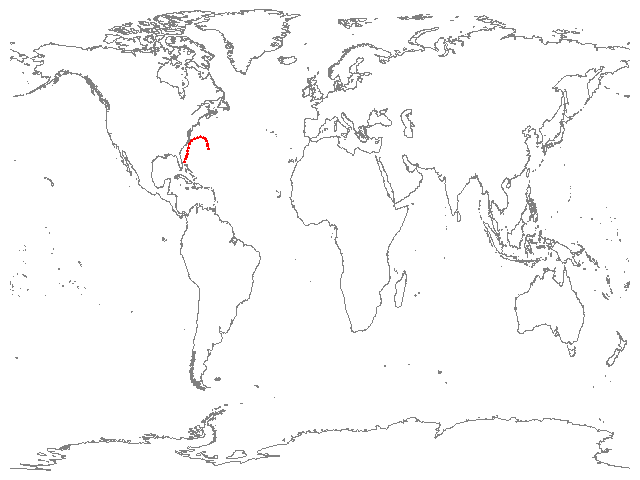
\includegraphics[width=0.33\linewidth]{plot01.png}
  \caption{The output plot for al012020.kml file. Shows the map representation of the cyclone from May 16 to May 21.}
  \label{fig:al012020}
\end{figure}
\begin{figure}[h]
  \centering
  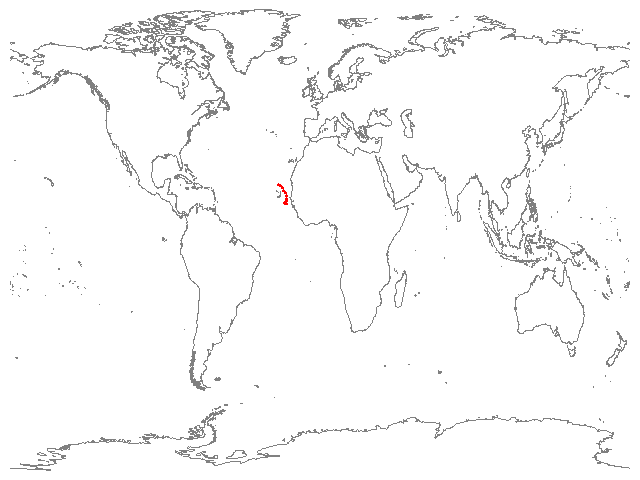
\includegraphics[width=0.33\linewidth]{plot10.png}
  \caption{The output plot for al102020.kml file. Shows the map representation of the cyclone from July 29 to August 02.}
  \label{fig:al102020}
\end{figure}
\begin{figure}[h]
  \centering
  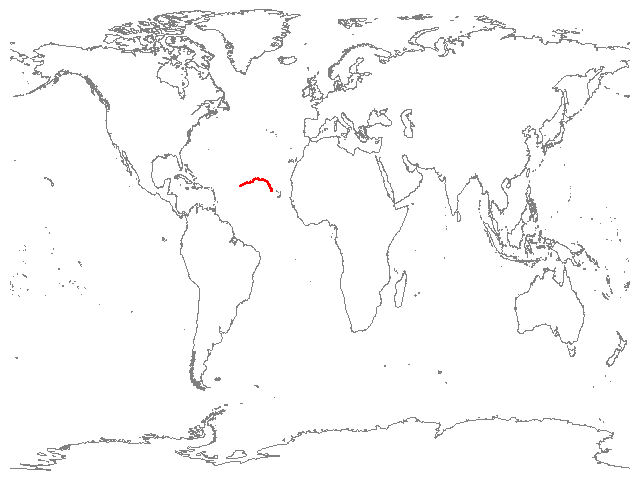
\includegraphics[width=0.33\linewidth]{plot21.png}
  \caption{The output plot for al212020.kml file. Shows the map representation of the cyclone from September 14 to September 19.}
  \label{fig:al212020}
\end{figure}
\clearpage



\section{Git usage}
During the development process, a conflict arose when merging the changes made in the \texttt{python-addon} branch with the main working branch. This conflict occurred in the \texttt{python-plot-script.py} file, which had been edited in both branches.

To resolve the conflict, the following steps were taken:

\begin{enumerate}
    \item Identified the conflicting sections within the \texttt{python-plot-script.py} file.
    \item Manually reviewed the changes made in both branches to understand the conflicting edits.
    \item Made necessary adjustments to the file to resolve the conflict, ensuring that the final version of the script incorporated the desired changes from both branches.
    \item Used Git commands to complete the merge and resolve the conflict:
    \begin{itemize}
        \item \texttt{git checkout main}: Switched to the main working branch.
        \item \texttt{git merge python-addon}: Merged the changes from the \texttt{python-addon} branch into the main branch.
        \item Resolved any merge conflicts within the \texttt{python-plot-script.py} file manually.
        \item \texttt{git add python-plot-script.py}: Added the resolved file to the staging area.
        \item \texttt{git commit -m "Resolved conflict in python-plot-script.py"}: Committed the changes with an appropriate message.
        \item \texttt{git push origin main}: Pushed the changes to the remote repository.
    \end{itemize}
\end{enumerate}

The final version of the \texttt{python-plot-script.py} file, which incorporated the resolved conflict, was successfully pushed to the remote repository and is provided below: This resolved version of the script ensured that all necessary changes were retained and integrated seamlessly into the project.

\subsection{python-plot-script.py Script}
\begin{lstlisting}[language=bash, caption={python-plot-script.py}]
import pandas as pd
import matplotlib.pyplot as plt
import os
import glob
import math
user_key= 27702

def plot_all_csv_pressure():
    path = os.getcwd()
    csv_files = glob.glob(os.path.join(path, '*.csv'))
    
    for f in csv_files:
        storm = pd.read_csv(f)
        storm['Pressure'].plot()
        plt.show()

def plot_all_csv_intensity():
    path = os.getcwd()
    csv_files = glob.glob(os.path.join(path, '*.csv'))
    
    for f in csv_files:
        storm = pd.read_csv(f)
        storm['Intensity'].plot()
        plt.show()
\end{lstlisting}
\end{document}
